\begin{figure}[htpb]
    \centering
    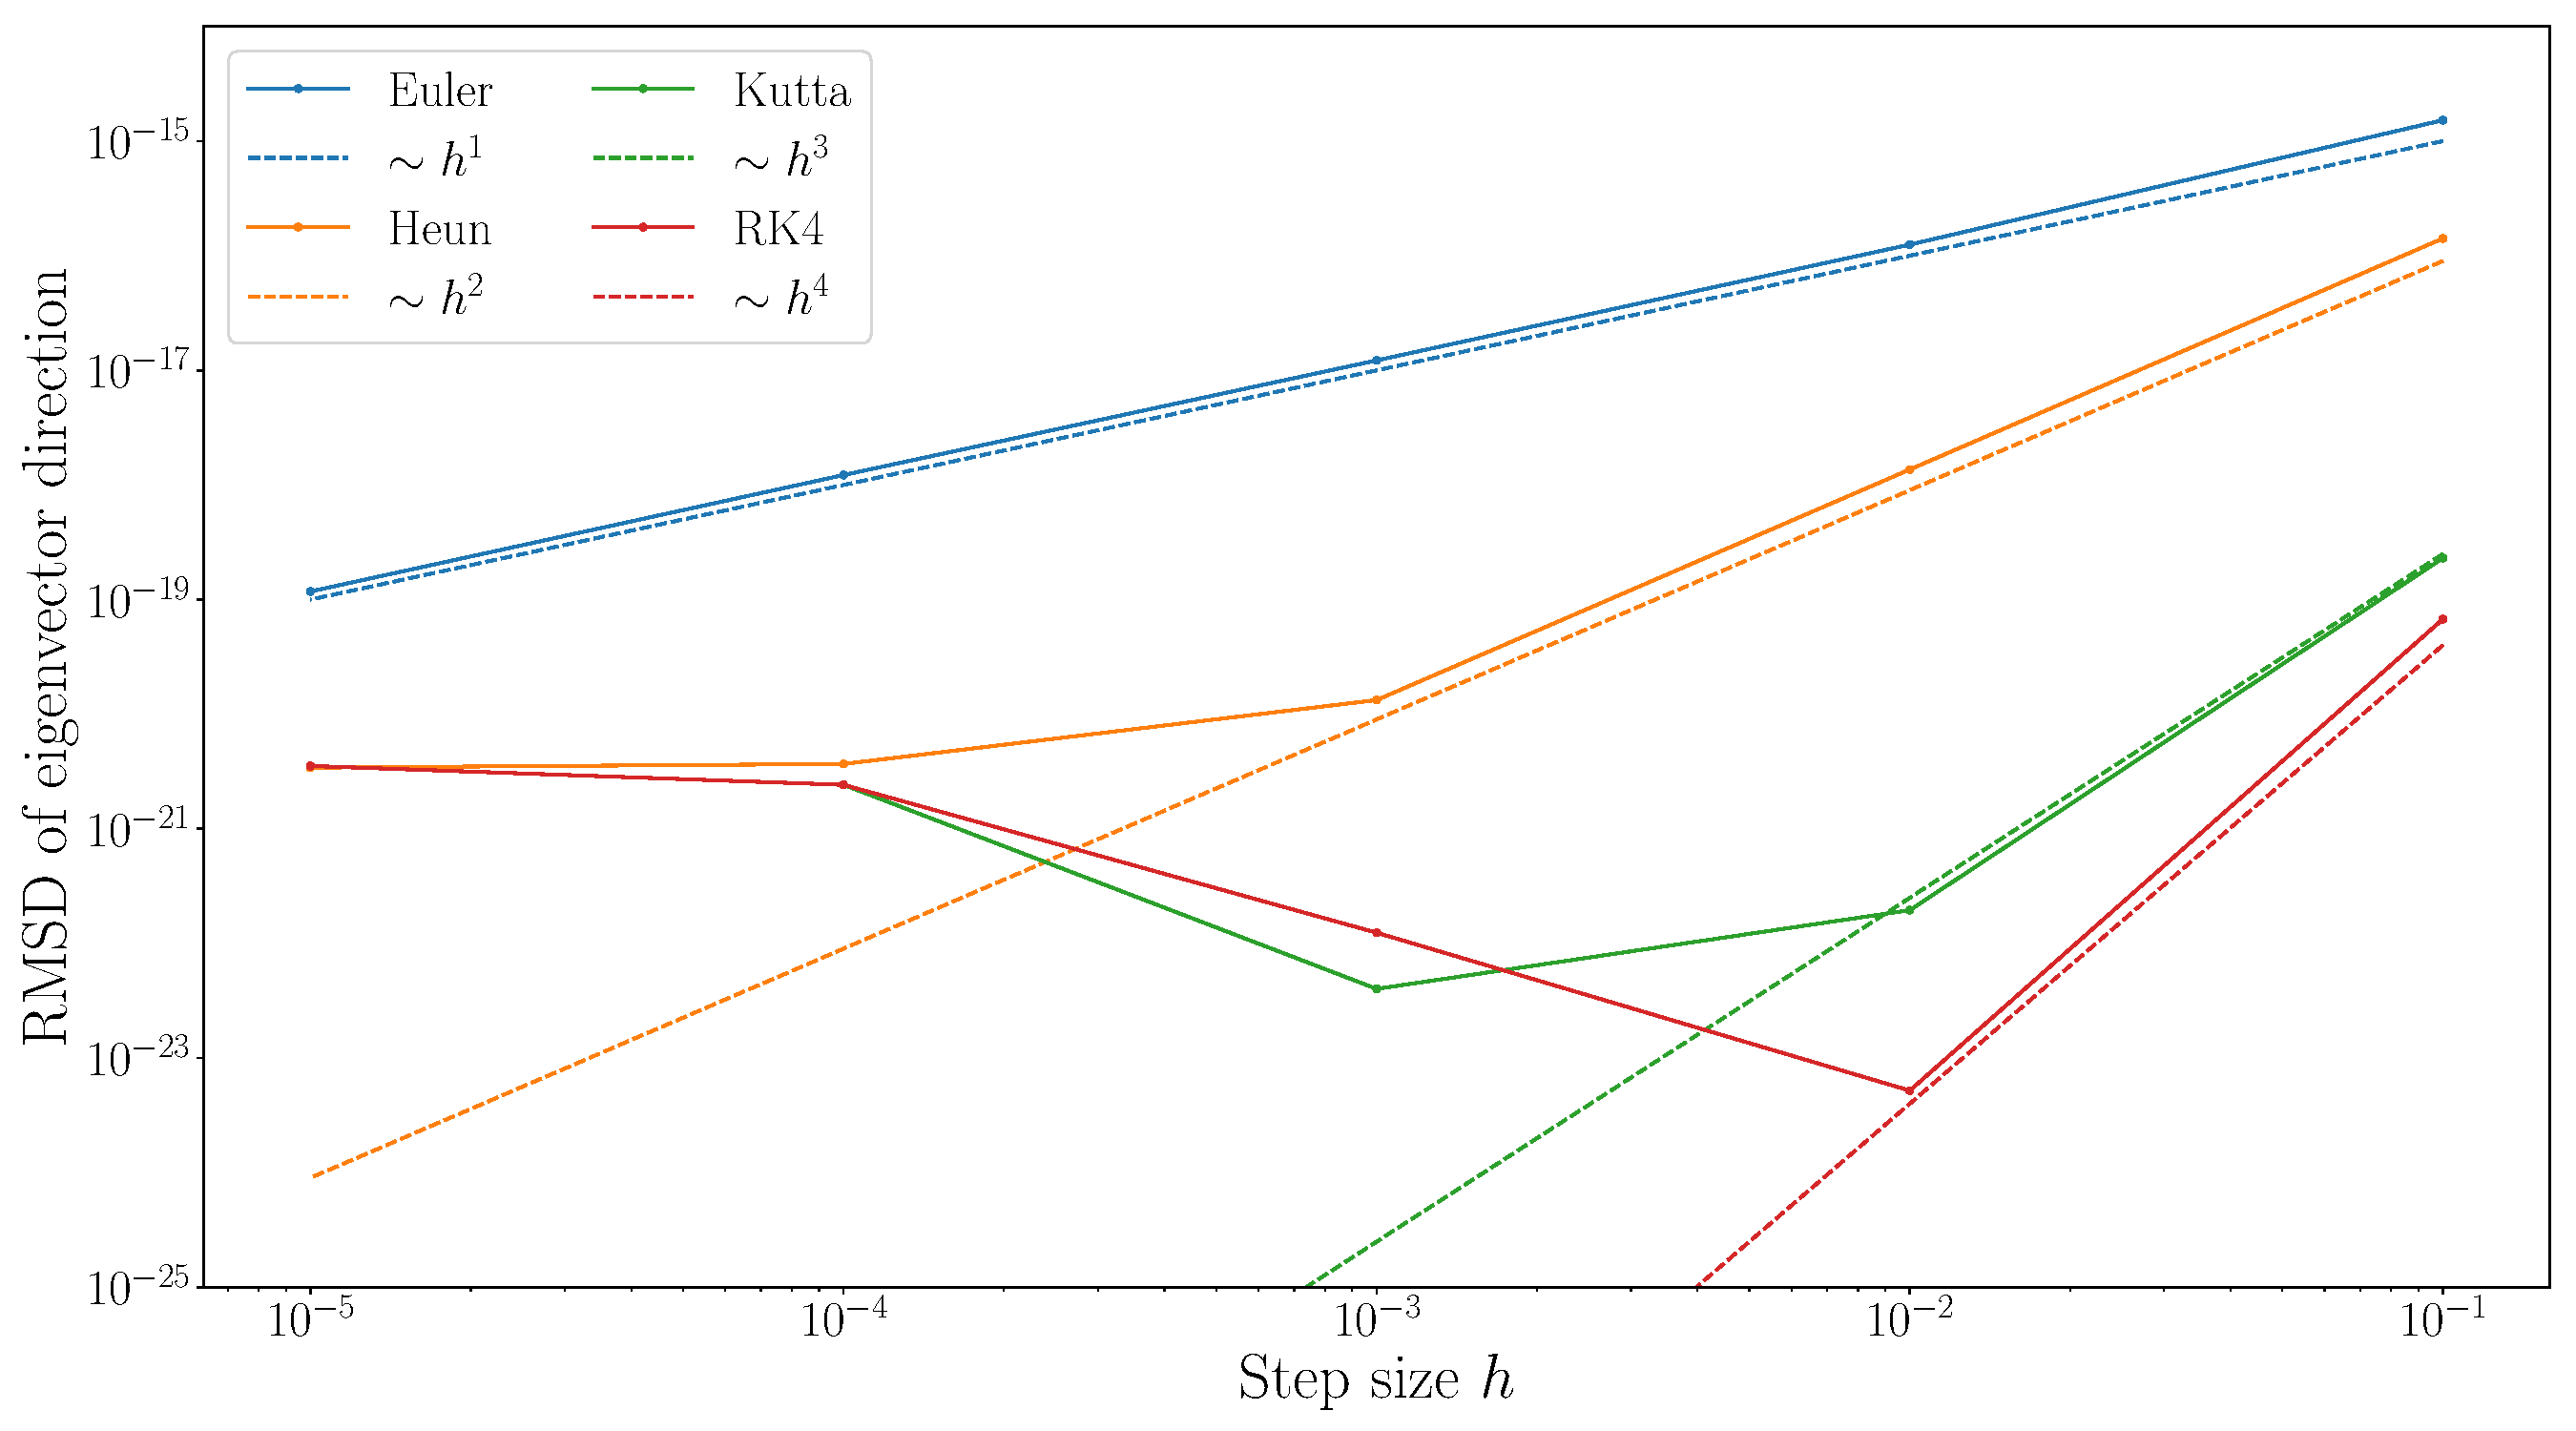
\includegraphics[width=0.8\linewidth]{figures/error_figures/xi2_errors_fixed_steplength.pdf}
    \caption[The identification process of strainlines which HOES BE AT BOI YE BOI BOII YE BOIIIII
    are local strain maximizers]{Illustration of the identification process of
        strainlines which are local strain maximizers.
        Local apices of $\overline{\lambda}_{2}(\gamma)$, the average of
        $\lambda_{2}$ over a curve $\gamma$, are found along a set $\mathcal{L}$
        of horizontal and vertical lines. The strainline segment
    $\gamma_{0}$ is identified as a local maximizer if it contains a locally
maximal $\overline{\lambda}_{2}$ value along at least one of the lines in
$\mathcal{L}$. Intersections of nearby strainlines, which fall within the dashed
ellipses, are included in the local comparison process for a given intersection
between a line in $\mathcal{L}$ and the strainline segment $\gamma_{0}$.}
    \label{fig:xi2err}
\end{figure}
